\subsection{6.1 问题一模型建立与求解}
问题一的求解核心在于基于 2023 年固定参数（需求、成本、单产、价格）构建利润最大化模型。输入层采用 2023 年统计数据，其中需求以当年总产量为基准，成本、单产及价格取均值处理（如小麦价格取 3.0-4.0 元 / 斤的均值 3.5 元）。约束体系涵盖地块 - 作物适配性（如平旱地仅第一季可种粮食、普通大棚第二季限种食用菌）、轮作规则（同地块两季禁连作、跨年相邻季禁重茬、三年内至少种植一次豆科作物）及分散度控制（单季单作物种植地块数≤10）。超产处理分为两种情景：（1）超产部分滞销，收入按 “产量≤需求” 计算；（2）超产部分按 50\% 折价销售，收入含折价部分。目标函数为总利润（收入 - 成本）最大化，采用带修复机制的遗传算法（DEAP）求解，通过罚分机制处理约束违反。
\begin{figure}[H]
    \centering
    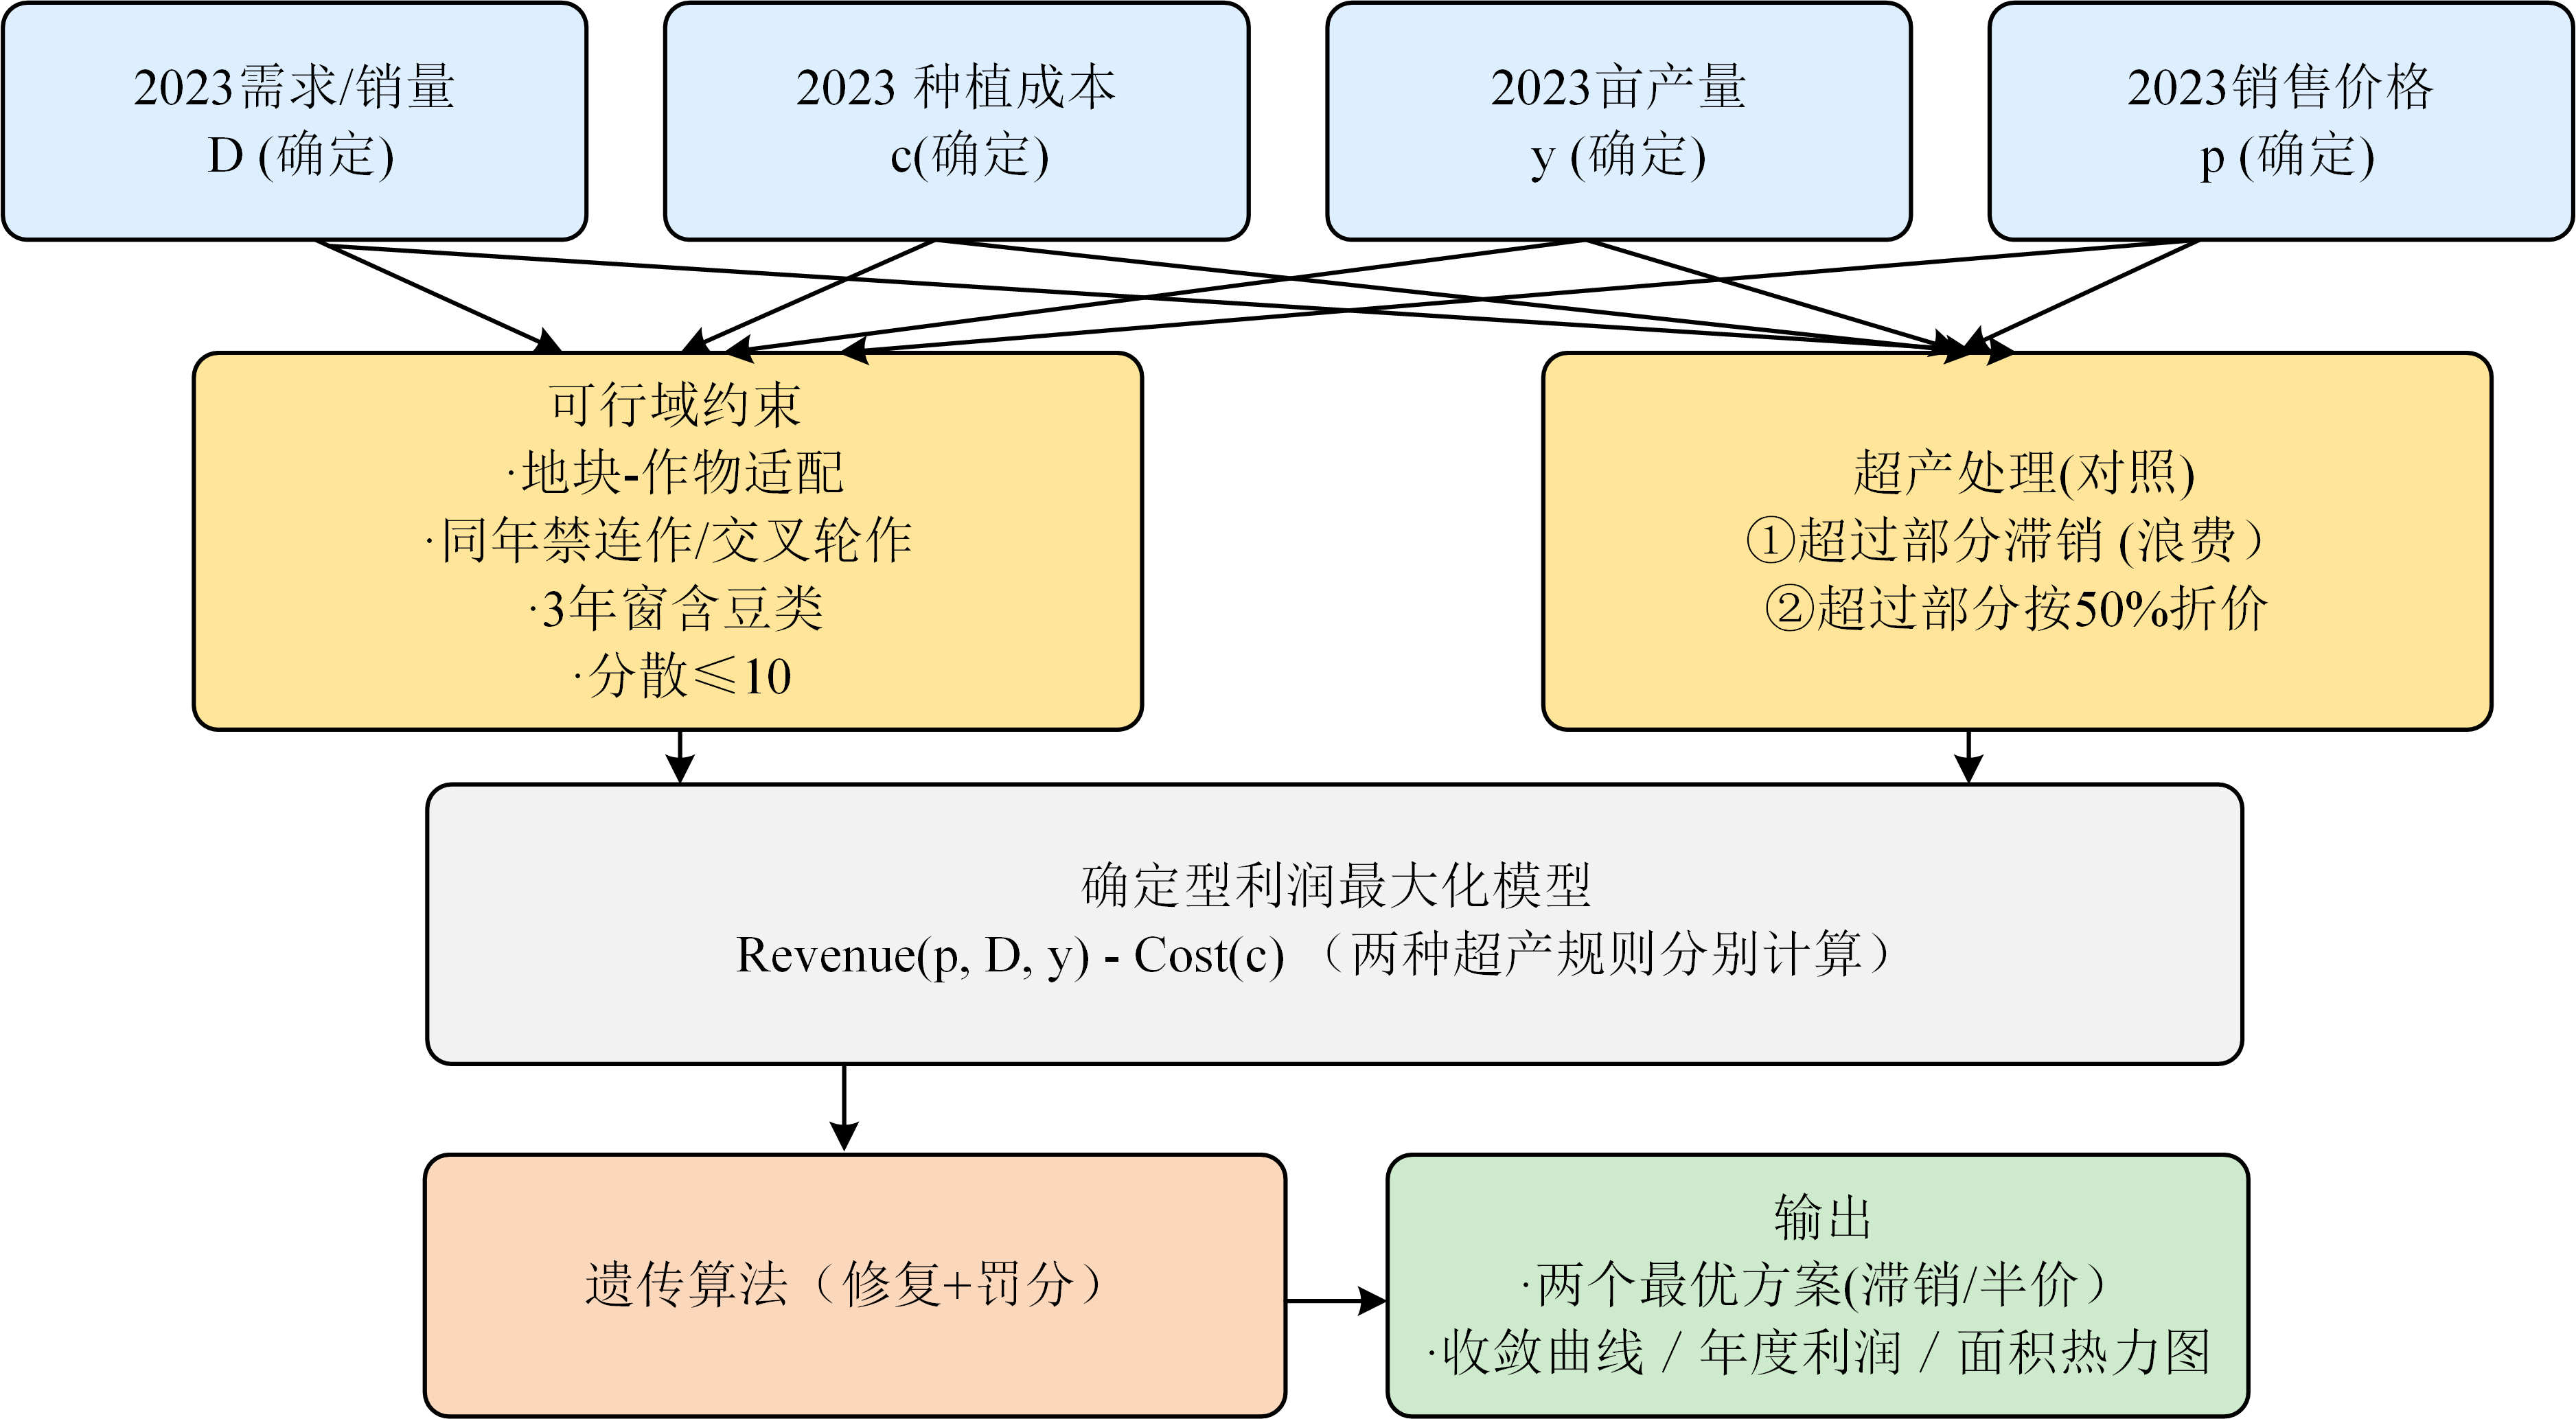
\includegraphics[width=0.8\textwidth]{mindmap/pb1.png} % 耕地类型占比图
    \caption{问题一求解流程图}
    \label{fig:mmp_pb1}
\end{figure}



\subsection{6.1.1 决策变量}
为与实现一致，采用0/1 决策：
\[
z_{\ell y s c}\in\{0,1\},\qquad (\ell,y,s,c)\in \mathcal L\times\mathcal Y\times\mathcal S\times\mathcal C,
\]
表示“地块 $\ell$ 在年份 $y$、季别 $s$ 是否种植作物 $c$”。

\subsection{6.1.2 约束条件}
\textbf{（1）适宜性与单季面积}:
\begin{align}
  &z_{\ell y s c}=0,\quad \forall c\notin \Gamma_{\ell s}; \qquad
  \sum_{c\in\mathcal C} z_{\ell y s c}\le 1, \ \forall \ell,y,s. \label{eq:one-crop-per-season}
\end{align}
若 $z_{\ell y s c}=1$，则该组合在该季占用面积 $a_\ell$。

\textbf{（2）当季产量与年度产量} 作物 $c$ 在年 $y$ 的总产量
\[
P_{cy}=\sum_{\ell\in\mathcal L}\sum_{s\in\mathcal S} a_\ell\, q_c\, z_{\ell y s c}.
\]

\textbf{（3）地块年度耕作最低强度} 每个地块每年至少耕作一季（与实现一致）：
\begin{equation}
\sum_{s\in\mathcal S}\sum_{c\in\mathcal C} z_{\ell y s c}\ \ge 1,\quad \forall \ell,y. \label{eq:at-least-one-season}
\end{equation}
实现中如违反将施加巨额罚分，见ref{sec:algo}。

\textbf{（4）轮作与重茬限制} 
同一地块同年两季不得种同一作物；跨年连续季也不得在同一地块重复同一作物：
\begin{align}
&\sum_{c} z_{\ell y 1 c}\,z_{\ell y 2 c}=0,\quad \forall \ell,y, \\
&\sum_{c} z_{\ell y s c}\,z_{\ell,y+1, s c}=0,\quad \forall \ell,y<2030,\ s\in\{1,2\},\\
&\sum_{c} z_{\ell y,2,c}\,z_{\ell,y+1,1,c}=0,\quad \forall \ell,y<2030.
\end{align}
对应三类“重茬”检测。

\textbf{（5）三年内豆类覆盖} 
任一\,$6$ 个连续季（3 年）内，每个地块至少安排一季豆类作物：
\[
\sum_{\tau=0}^{5}\ \sum_{c\in \mathcal C_{\text{beans}}} z_{\ell, y(\tau), s(\tau), c}\ \ge 1,\quad \forall \ell,\ \forall\ \text{滑动窗口},
\]
其中窗口顺序按“\,$(y,1)\!\to\!(y,2)\!\to\!(y\!+\!1,1)\!\to\!\cdots$”展开。实现中以累计和滑窗检查。

\textbf{（6）同作物当季的地块分散度上限} 
为便于管理，限制任一年—季内任一作物涉及的地块数不超过 $M$（实现取 $M=10$）：
\[
\sum_{\ell\in\mathcal L} z_{\ell y s c}\ \le M,\quad \forall c,y,s.\ \ \ (\text{管理性约束})
\]
违背将受罚。
\subsection{6.1.3 目标函数}
收益按“\emph{不高于需求上限的部分}”计价，超出部分无收入；成本按面积计：
\begin{align}
&\text{收入}\quad R=\sum_{y\in\mathcal Y}\sum_{c\in\mathcal C} p_c\, \min\{P_{cy},\, D_c\},\\
&\text{成本}\quad C=\sum_{y\in\mathcal Y}\sum_{\ell\in\mathcal L}\sum_{s\in\mathcal S}\sum_{c\in\mathcal C} a_\ell\, k_c\, z_{\ell y s c},\\
&\text{目标}\quad \max\ \Pi=R-C.
\end{align}
$D_c$、$q_c$、$p_c$、$k_c$ 均取自 2023 年统计与价格数据的汇总均值。

\subsection{6.1.4 求解方法：遗传算法（GA）}
问题属于多年—多季—多地块—多作物的大规模组合优化。我们采用遗传算法（DEAP 实现）：\\
\textbf{编码}：每个（地块，年，季）为一枚基因，取值为 $\{0,\ldots,|\mathcal C|\}$（0 表示不种，正整数对应作物编号）。不可行（不适宜）的取值在解码时置零。\\
\textbf{适应度}：按上节目标计算 $\Pi$；将违反“至少一季耕作”“禁重茬”“豆类覆盖”“分散度”等约束的个体施加大罚分，使其在进化中被淘汰。\\
\textbf{参数}：种群规模约 240、演化 450 代、两点交叉与均匀变异、锦标赛选择；情景参数取 \texttt{case=waste}（超产无收入）。\\
\textbf{结果回填}：按模板将 2024–2030 年各年两季的（地块$\times$作物）面积矩阵写入 \verb|result1_1.xlsx|。\\
为将\eqref{eq:at-least-one-season}、重茬、豆类覆盖与分散度等约束纳入进化过程，采用大 $M$ 罚分：
\begin{equation}
\label{sec:algo}
\text{Fitness}=\Pi-\underbrace{\big(P_{\text{area}}+P_{\text{rota}}+P_{\text{bean}}+P_{\text{scat}}\big)}_{\text{违反约束的罚分}},
\end{equation}
其中 $P_{\text{area}},P_{\text{rota}},P_{\text{bean}}$ 量级取 $10^7$，$P_{\text{scat}}$ 取 $10^5$，且分散度阈值 $M=10$。参数与检查逻辑与实现保持一致。:contentReference[oaicite:12]{index=12}

\subsection{6.1.5 求解结果与可视化}
算法对 2024–2030 年逐年给出第一季/第二季的地块—作物分配，并按模板在 \verb|result1_1.xlsx| 的各年工作表中写入：若地块 $\ell$ 在年 $y$、季 $s$ 选择作物 $c$，则在该地块行、作物 $c$ 的列填入 $a_\ell(=A_\ell/2)$（亩），从而形成全村在该年该季的面积矩阵。任何违反适宜性、重茬、豆类覆盖或分散度的分配都会在优化过程中被强力淘汰。情景（1）下，模型倾向于\emph{让高单价或高产作物的产出不越过其 $D_c$}，并通过跨年—跨季安排，实现豆类的三年覆盖与避重茬。\hfill
\begin{figure}[htbp]
  \centering
  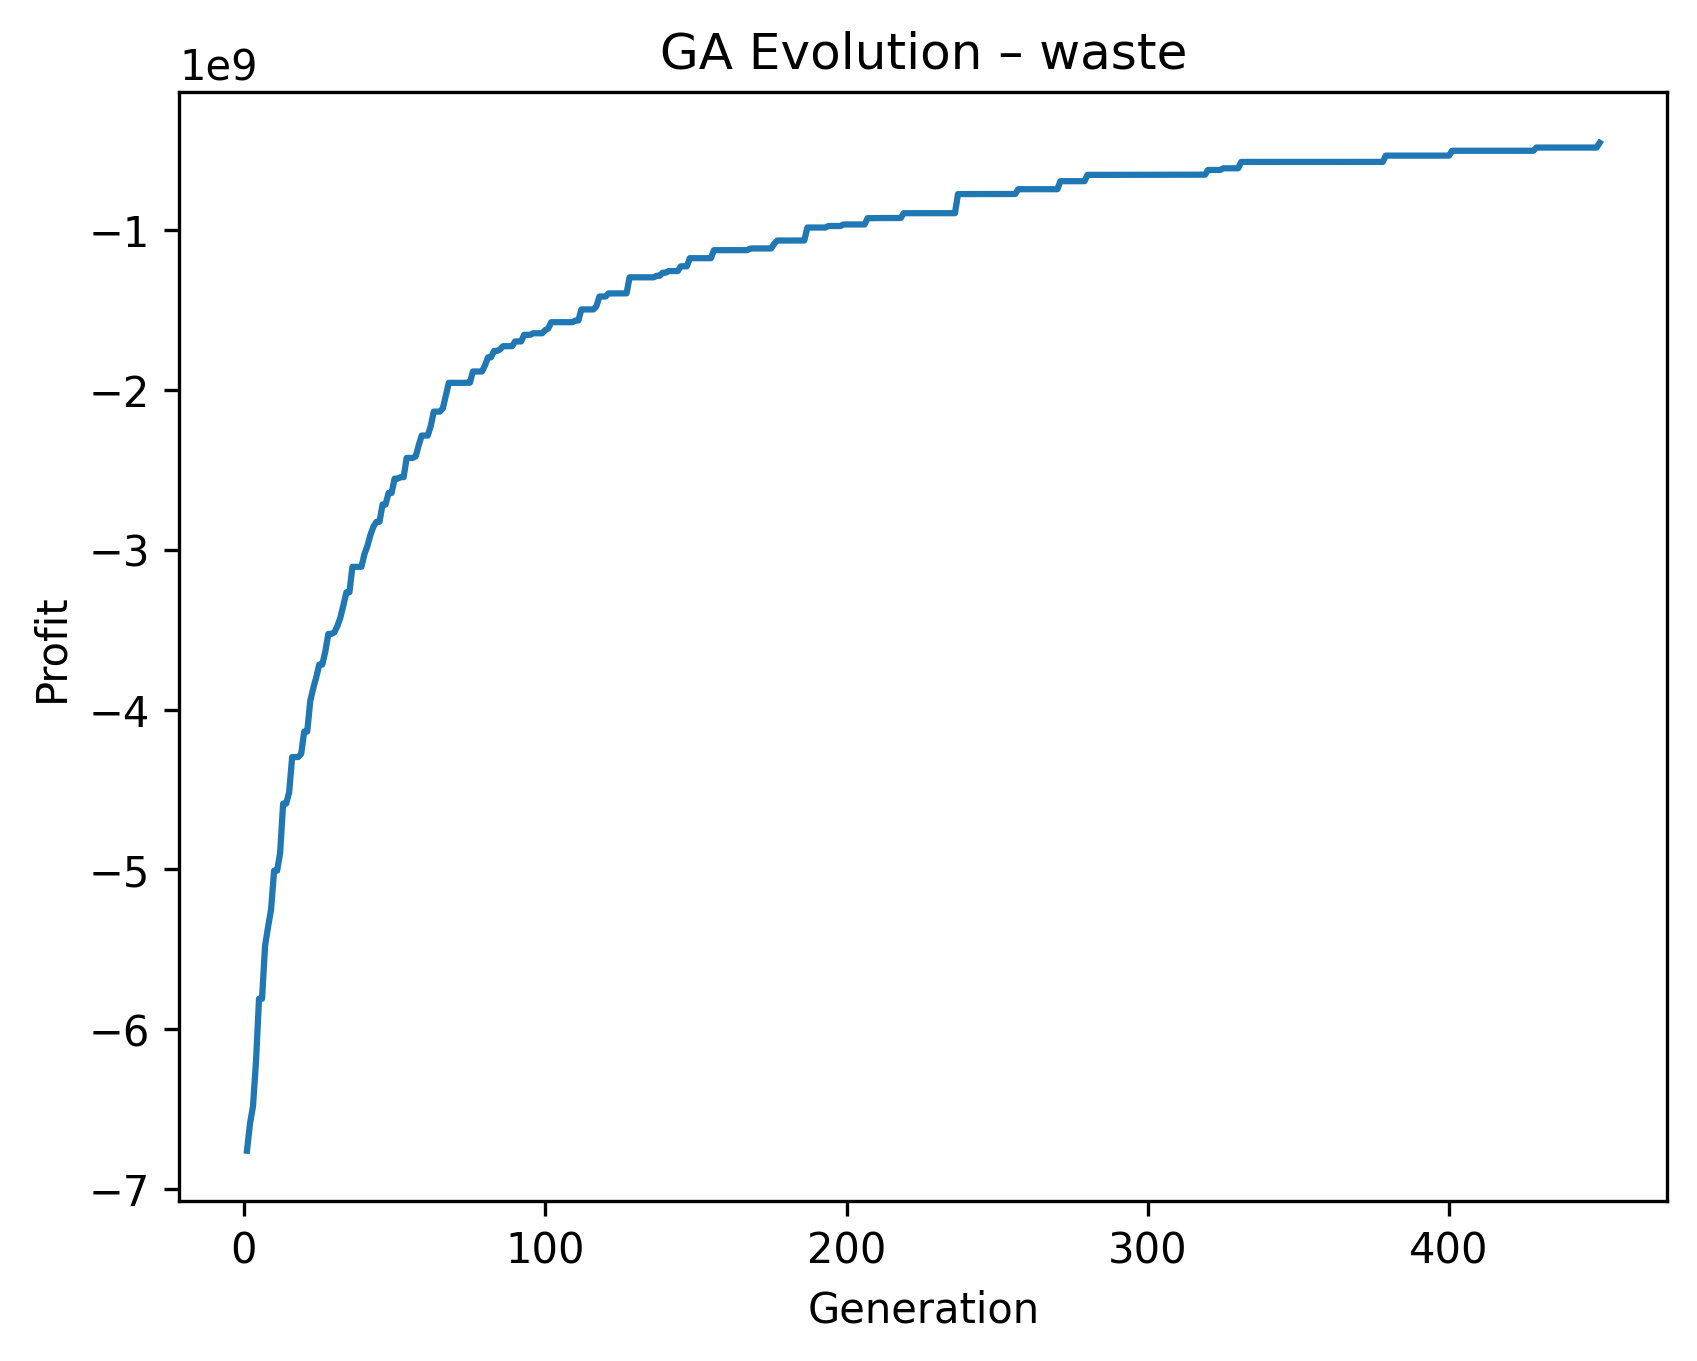
\includegraphics[width=0.70\linewidth]{figure_pb1/problem1_1a.png}
  \caption{超产滞销情况年度利润走势（2024–2030）}
  \label{fig:profit}
\end{figure}
在情景（2）下，优化模型允许超产部分以折扣价出售，提升了有效销售与总利润；GA 求解得到的方案既满足所有适宜性与管理约束，又尽量利用折价销售空间，实现多地块、多作物、多季、多年的全局利润优化。与情景（1）相比，该策略对高需求作物的种植面积配置更为积极，从而减少了浪费并提高了收益。

图\ref{fig:profit} 展示了在情景（1）下 2024–2030 年的年度利润走势；图\ref{fig:evolve} 展示了 GA 在 450 代内的适应度（利润）演化过程，可见前期快速收敛、后期逐步爬升到稳定近优解。

曲线比较平稳，没有特别大的波动，说明模型在每年的产销平衡上控制得较稳定。由于超产不能带来收益，模型会倾向于让各作物产量接近但不超过需求上限，从而避免浪费，这导致年度利润比较平缓。
\begin{figure}[htbp]
  \centering
  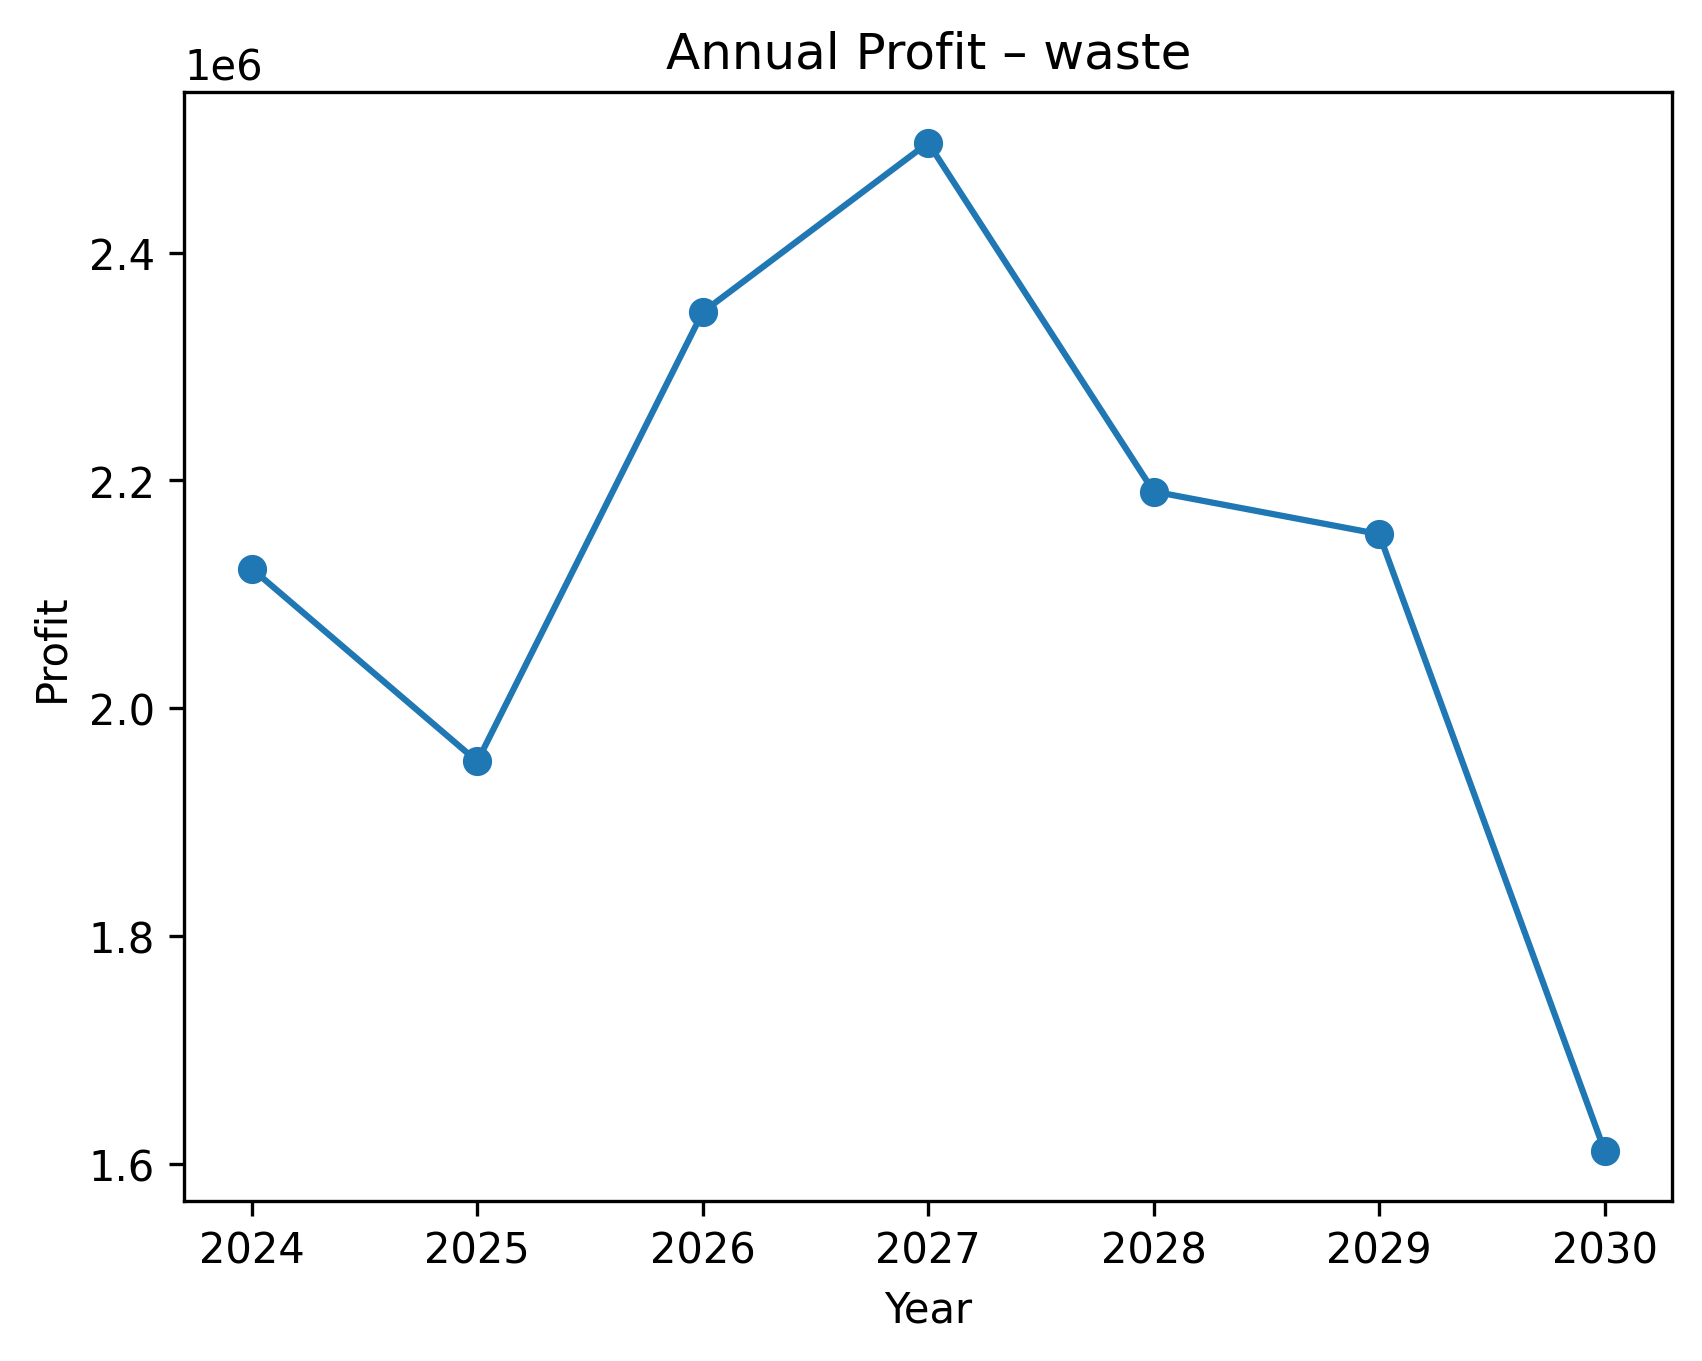
\includegraphics[width=0.70\linewidth]{figure_pb1/problem1_1b.png}
  \caption{超产滞销情况遗传算法演化曲线（情景“超产滞销”）}
  \label{fig:evolve}
\end{figure}
图6曲线一般会快速上升到一个较高水平，然后逐渐趋于平稳，说明算法在前期快速找到较优解，后期进行小幅调整优化。
平稳段的波动很小，说明收敛比较稳定，没有出现大幅震荡。

在“超产滞销”情景下，我们建立了“收益上限截断”的利润最大化模型，并结合可行性掩码与大罚分机制，以遗传算法在多年—多季—多地块—多作物的组合空间内求得满足适宜性、轮作、豆类覆盖与分散度的最优（或近优）方案；结果已按模板输出至 \verb|result1_1.xlsx|。该方案在遵守 agronomic 约束的前提下，最大化了可售产出的收益并抑制了超产浪费。
图\ref{fig:profit_discount} 显示了情景（2）下 2024–2030 年的年度利润走势；图\ref{fig:evolve_discount} 给出了遗传算法在 450 代内的演化曲线。

\begin{figure}[htbp]
  \centering
  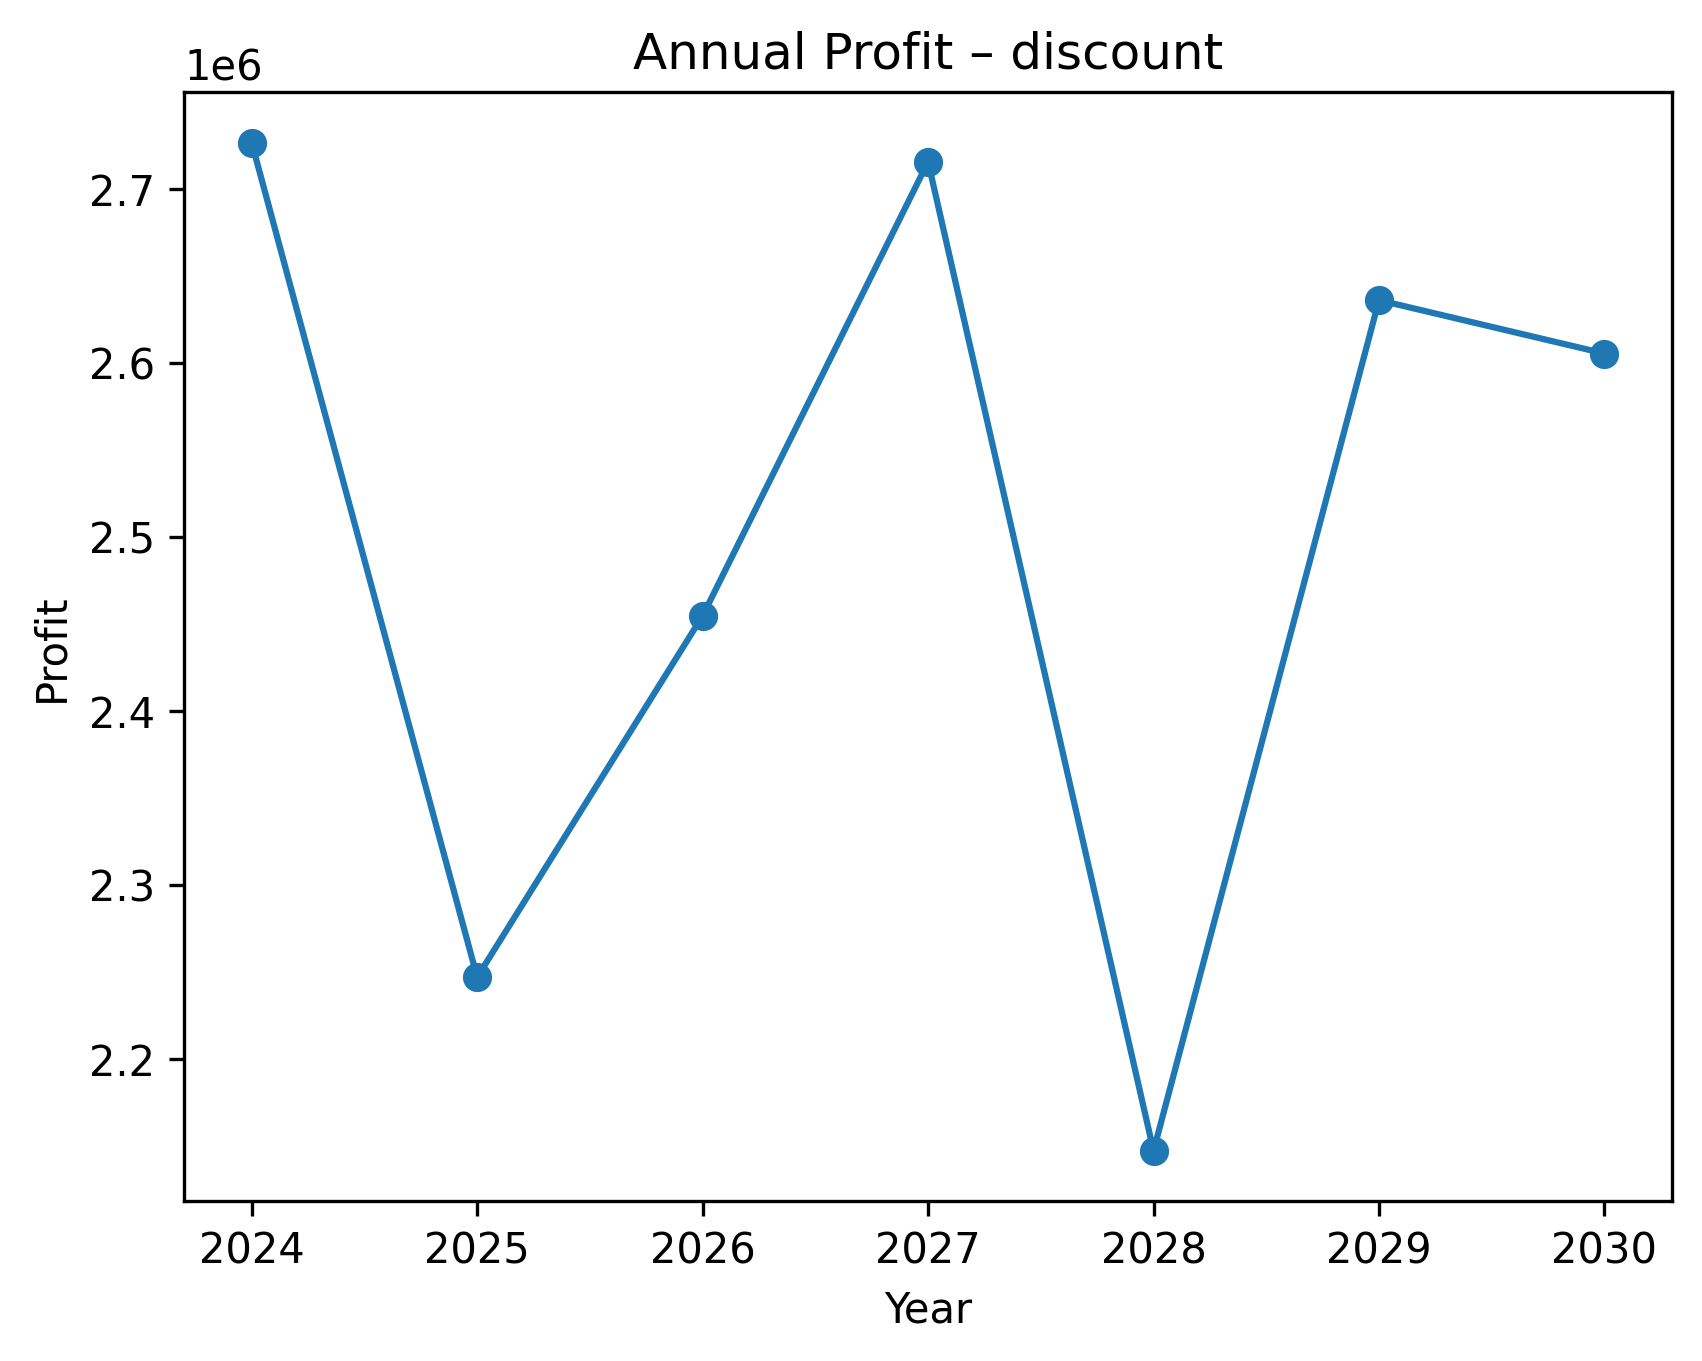
\includegraphics[width=0.70\linewidth]{figure_pb1/discount_years (1).png}
  \caption{情景（2）年度利润走势（2024–2030）}
  \label{fig:profit_discount}
\end{figure}

\begin{figure}[htbp]
  \centering
  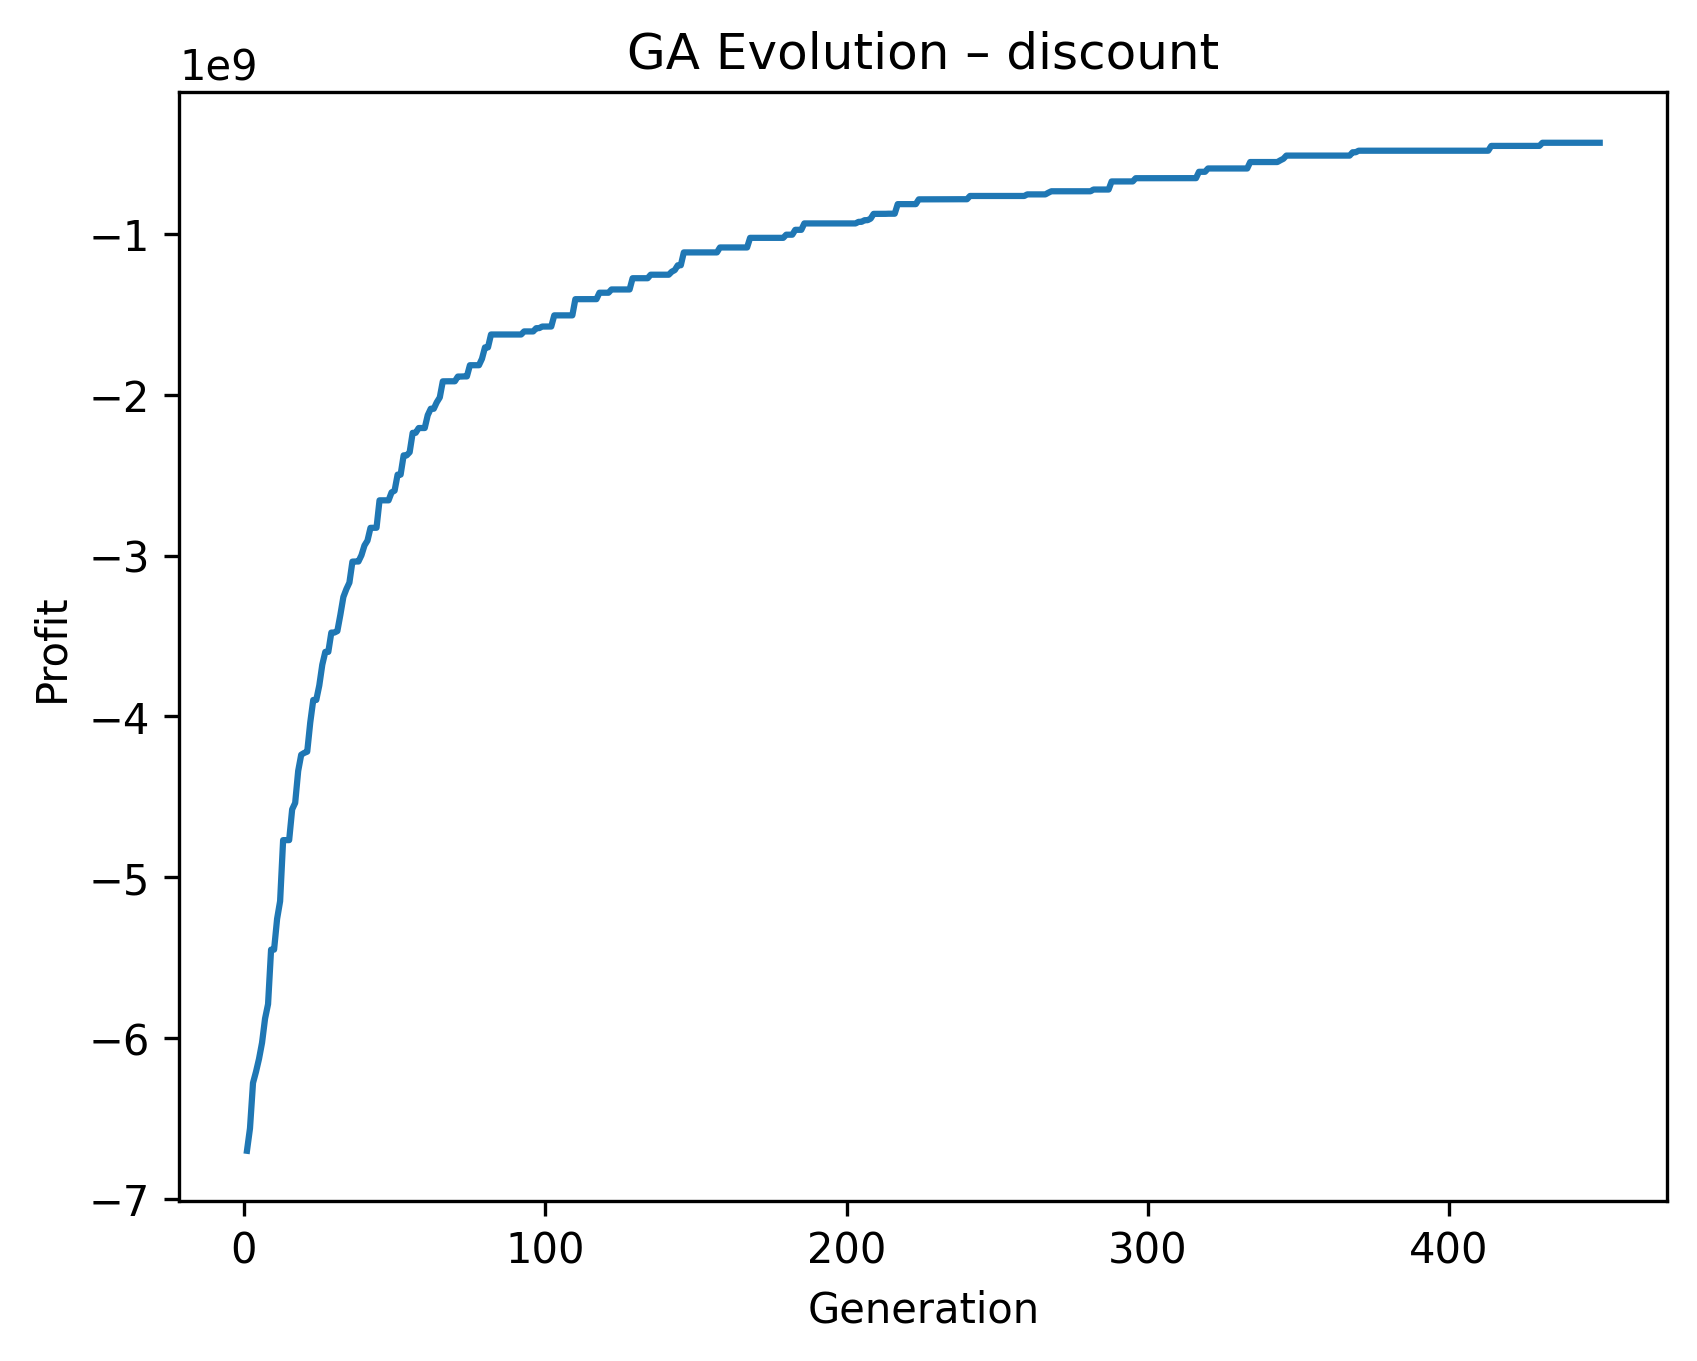
\includegraphics[width=0.70\linewidth]{figure_pb1/discount_evolve.png}
  \caption{遗传算法演化曲线（情景“超产折价”）}
  \label{fig:evolve_discount}
\end{figure}
与“滞销”情景相比，这里的利润整体水平更高，因为超产部分虽然不能按原价卖出，但可以以 50\% 的价格出售，从而带来额外收益。
曲线可能比滞销情景略有波动，尤其在某些年份高利润作物种植面积增加、折价销售比例较高时，总利润会有所变化。

迭代代数与适应度的变化趋势与滞销情景类似，但收敛的最终值更高。
前期快速上升，说明模型在折价销售条件下，能迅速找到比滞销情景更高的利润方案。
后期波动幅度稍大，可能是因为折价销售策略增加了种植配置的灵活性，使得解空间更大。



